\section{Exceptional Control Flow}

\section*{Interrupt sources}
\begin{itemize}
  \item Perfipherals signal to CPU that an event needs immediate attention
  \item Can alternativly be generated by software request
  \item Asynchronous to instruction execution
\end{itemize}

\section*{System exceptions}
\begin{itemize}
  \item Reset
  \item NMI
  \item Faults
  \item System Level Calls
\end{itemize}

Restart of processor\\
Non-maskable Interrupt (cannot be ignored) Undefined instructions OS calls - Instructions SVC and PendSV

\begin{center}
\begin{tabular}{|c|c|c|c|}
\hline
\multicolumn{3}{|l|}{\begin{tabular}{l}
PRIMASK \\
- Single bit controlling all maskable interrupts \\
\end{tabular}} & 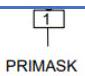
\includegraphics[width=\linewidth]{images/2024_12_29_79e6b22f503fb7b4f718g-11}
 \\
\hline
\begin{tabular}{l}
- Disable \\
- Enable \\
\end{tabular} & set PRIMASK clear PRIMASK & \begin{tabular}{l}
Assembly \\
CPSID ${ }^{1)}$ CPSIE ${ }^{1)}$ \\
\end{tabular} & C disable\_irq(); - enable\_irq(); \\
\hline
\multicolumn{4}{|l|}{On reset PRIMASK $=0 \quad \rightarrow$ enabled} \\
\hline
\end{tabular}
\end{center}

\section*{Storing the context}
Interrupt event can take place at any time

\begin{itemize}
  \item E.g. between TST and BEQ instructions
  \item ISR call requires automatic save off lags and caller saved registers
\end{itemize}

ISR call

\begin{itemize}
  \item Stores xPSR, PC, LR, R12, R0-R3 on Stack
  \item Stores EXC\_RETURN to LR
\end{itemize}

ISR Return

\begin{itemize}
  \item Use BX LR or POP \{..., PC\}
  \item Loading EXC Return into PC
  \item Restores RO-R3, R12, LR, PC and xPSR from Stack
\end{itemize}

\section*{Polling}
Periodic query of status information

\begin{itemize}
  \item Reading of status registers in loop
  \item Synchronous with main program
  \item Advantages
  \item Simple straightforward
  \item Implicit synchronisation
  \item Deterministic\\
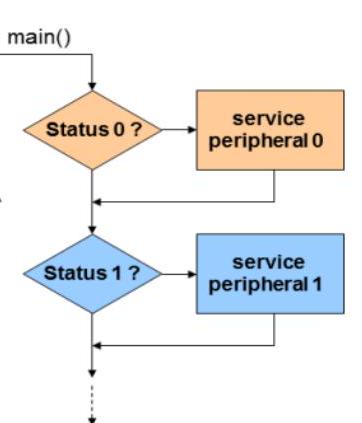
\includegraphics[width=\linewidth]{images/2024_12_29_79e6b22f503fb7b4f718g-11(1)}
  \item No additional interrupt logic required
  \item Disadvantages
  \item Busy wait -> wastes CPU time
  \item Reduced throughput
  \item Long reaction time
  \item No synchronization
  \item Difficult debugging\\
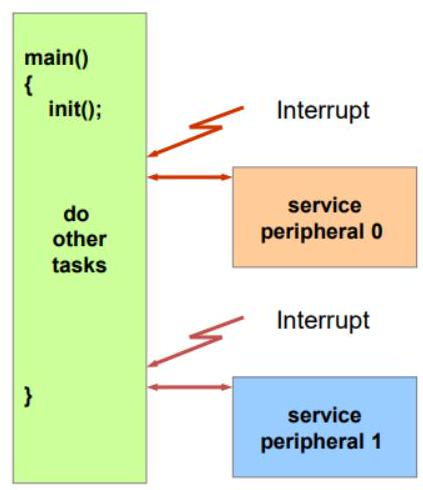
\includegraphics[width=\linewidth]{images/2024_12_29_79e6b22f503fb7b4f718g-11(2)}\\
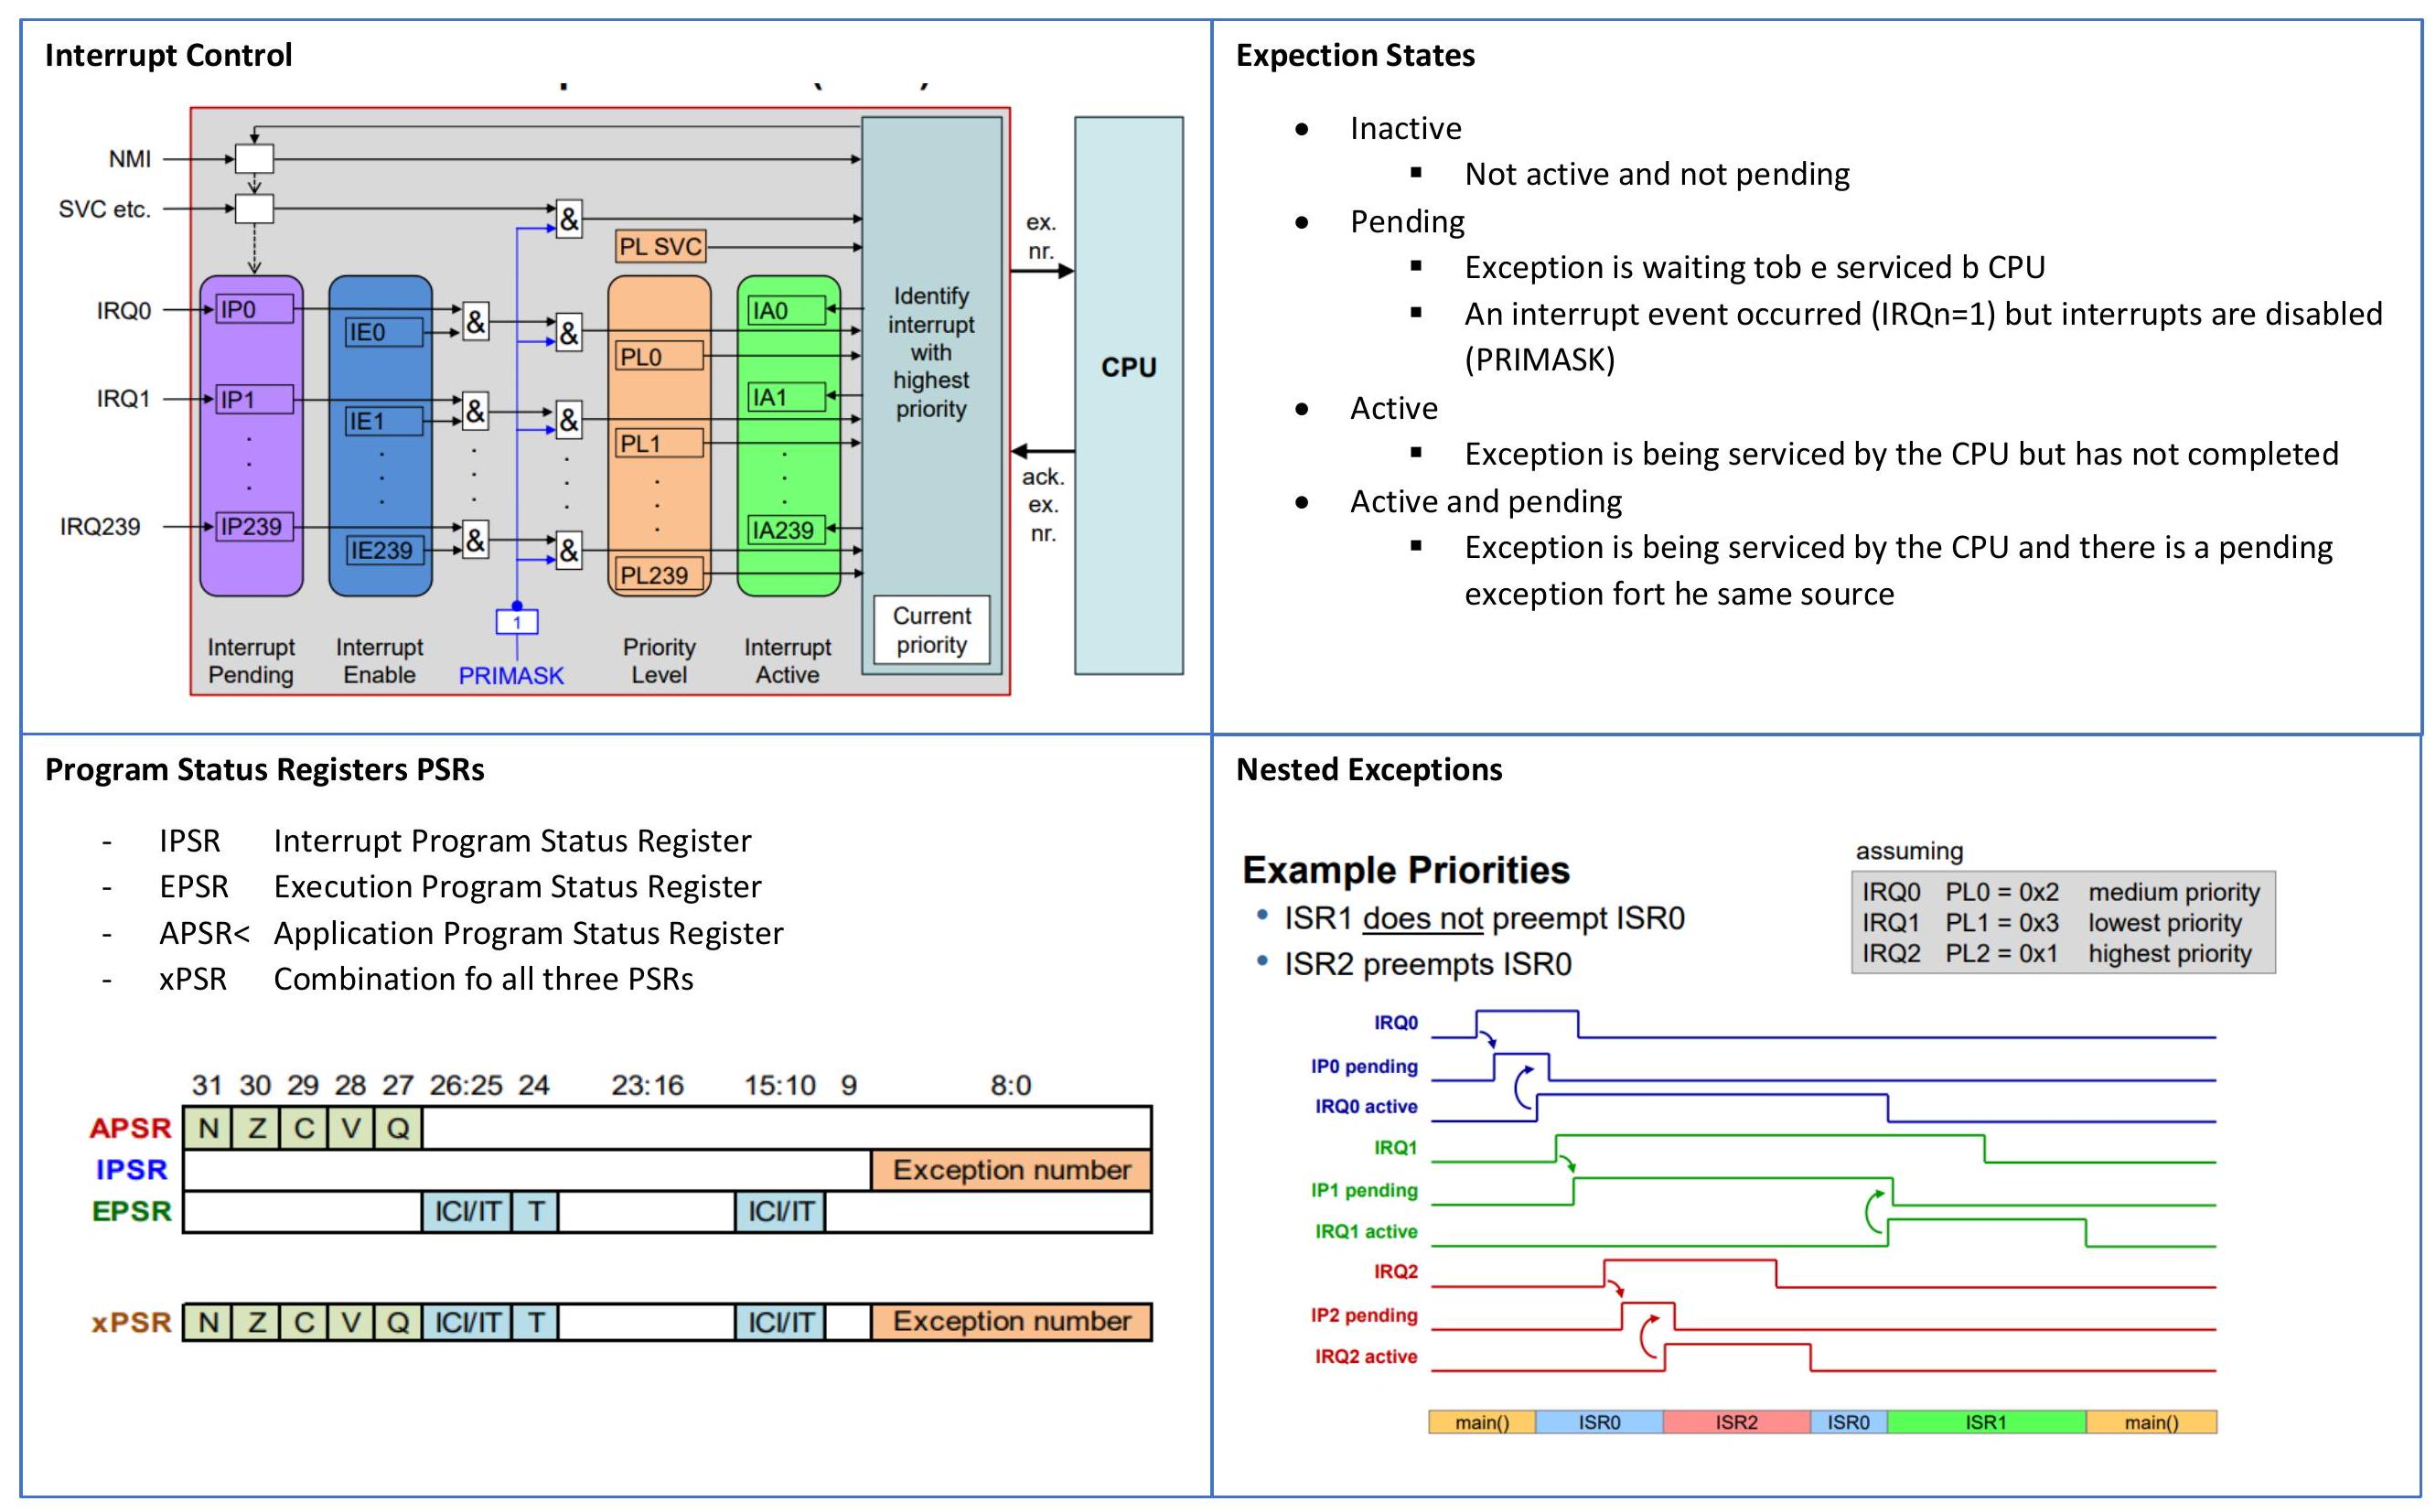
\includegraphics[width=\linewidth]{images/2024_12_29_79e6b22f503fb7b4f718g-12}
\end{itemize}